\documentclass[11pt]{article}
\usepackage[margin=1in]{geometry}
\usepackage{amsmath,amssymb,amsfonts,amsthm}
\usepackage{graphicx,booktabs,url,xcolor}
\usepackage[hidelinks]{hyperref}
\newcommand{\lean}[1]{\textsf{\footnotesize #1}}
\newtheorem{theorem}{Theorem}
\newtheorem{definition}{Definition}

\title{Upgrading Communication Without Retraining Every Agent:\\ Legacy-View Emulation for Mixed-Version MARL\\[4pt]
\large DRAFT v2 (04/10/2026) --- every number is a report line cited in \texttt{PAPER\_E3\_LEGACY\_VIEW\_CLAIM\_TABLE\_20261004.md}}
\date{}

\begin{document}
\maketitle

\begin{abstract}
A deployed multi-agent team cannot always retrain every agent when its communication protocol is upgraded. Agents that keep the old
policy (OLD) were trained on the view the old protocol built from its message history; a new protocol with the same packet format can
change that view at nearly every step. We study legacy-view emulation: the new protocol carries, or reconstructs, exactly the view the
frozen receivers were trained on. We give two implementations of one contract. A base-packet decoder in which every node rebuilds the
legacy view from local information only is exact by theorem on the same physical trajectory (mechanised in Lean). A zero-byte emulator
that uses only what OLD receivers already hear is exact if and only if a coverage condition holds, which we prove and measure (it failed
on $3.8\cdot10^{-5}$ of OLD agent-steps). In a mixed fleet of eight OLD and eight NEW traffic-signal agents, emulation recovers system
performance relative to fallback and to running OLD agents on the new channel without emulation; against retraining the OLD receivers
we detect no difference. Exact views do not imply unchanged returns: NEW agents change the trajectory, and per-agent non-inferiority of
OLD agents was not established.
\end{abstract}

\section{Introduction}
A communication upgrade can preserve the packet schema while changing the cached and relayed observations on which a learned receiver
relies. In a fleet that is upgraded in stages, some agents (NEW) are retrained for the new channel while others (OLD) keep frozen
weights, because retraining them is costly, slow to certify, or not permitted. The OLD agents' policies are feed-forward functions of a
\emph{view}: a table that the old protocol assembles from the history of packets each node has received (who sent what, how fresh it is,
which copies were relayed). The new protocol changes that history even when every packet still fits the old format, so the OLD view
changes. In our testbed, the naive design --- NEW senders put their new relay table into the unchanged 25-byte packet --- changes the OLD
view at every one of 3200 OLD steps per seed and changes 1048--1940 actions (Section~\ref{sec:exact}).

This paper asks a narrow question: can the new protocol deliver to OLD receivers exactly the view they were trained on, and what does
that buy in a mixed fleet? Our contributions are:
\begin{enumerate}
\item \textbf{A contract.} The legacy view is a function of the history; the upgraded protocol meets the contract at node $i$ if a causal,
local decoder $D_i$ applied to the node's upgraded state returns that function, $D_i(T^U_i(h_t)) = v^K_i(h_t)$ for every history $h_t$.
\item \textbf{Two implementations with different guarantees.} A base-packet decoder that is exact on every trajectory under a nesting
condition (Lean, Theorem~\ref{thm:dec}), and a zero-byte receiver-side emulator that is exact if and only if a measurable coverage
condition holds (Lean, Theorem~\ref{thm:emu}).
\item \textbf{A mixed-fleet evaluation} with registered endpoints, against fallback, rollback, plain deployment, and update-permitted
references (fine-tuning and positive-congruent training of the OLD receivers), with the byte cost of every arm.
\end{enumerate}
We do not claim that exact views protect OLD agents' returns: NEW agents change the physical trajectory that OLD agents act in, and our
per-agent analysis does not establish non-inferiority (Section~\ref{sec:e13}).

\section{Setting}\label{sec:setting}
\paragraph{Team and task.} Sixteen traffic-signal agents on a $4\times4$ CityFlow grid; an episode has 26 decision steps. Performance is
the system queue, reported as a percentage gain over ZTEAM, a compiled-silent student distilled from the same teacher that uses no
messages (a strict bar: a receiver that is worse than ZTEAM would have been better off ignoring its channel).
\paragraph{Channels.} Agents broadcast 25-byte packets. The legacy channel K1 delivers one packet per receiver per step on a public
schedule and relays through a per-node table: each entry is a sender's freshest known measurement with its measurement time. The
upgraded channels deliver more packets per step at i.i.d.\ capacities: U1 reorders adaptively; U2 preserves order and delivers a superset
of the K1 schedule at every step (\emph{nesting}). Delivered bytes per episode: 78\,058 on U1/U2 versus 10\,400 on K1.
\paragraph{Versions.} OLD receivers are the checkpoints trained on K1; NEW agents are trained on the upgraded channel. Layout D (primary)
places the eight OLD agents on a checkerboard; layout C (secondary) places them in a contiguous block.

\begin{definition}[K1 view]
For receiver $i$ at step $t$, $v^K_i(h_t)$ is, for every sender $j$ the legacy table lists, the freshest legacy entry of $j$ that the K1
schedule would have delivered or relayed to $i$ by $t$, with its measurement time.
\end{definition}

\section{Legacy-view emulation}
\subsection{Base-packet decoder (exact)}
NEW senders additionally broadcast a base packet carrying their legacy (K1) relay state; every node, NEW or OLD, runs the legacy update
on the base packets it decodes.
\begin{theorem}[decoder = reference; Lean \lean{dec\_eq\_ref}, \lean{dec\_wire\_eq\_ref}]\label{thm:dec}
If the upgraded delivery nests the legacy schedule ($S_t(i)\subseteq D_t(i)$ for all $t,i$), then every node running its local update on
the base packets it receives holds exactly the K1 cache and view of the reference run, at every step, on the same physical trajectory
(full-precision timestamps). With the age field saturated at $c$ steps the decoder is exact for every step $t\le c+1$.
\end{theorem}
The Lean module (\lean{LeanMarlLegacyViewDecoderV1}; 21 audited theorems, standard axioms only) also shows that the hypothesis is not
vacuous (\lean{miss\_breaks}: one missing scheduled packet changes the view; \lean{nesting\_satisfiable}, including strict nesting) and
that saturation can flip the merge in general (\lean{saturation\_can\_flip}). Beyond $t=c+1$ (26 steps, $c=14$) exactness of the 4-bit
wire format is an \emph{empirical} result (Section~\ref{sec:exact}). Cost: one extra base packet decoded per node per step, 1\,300~B of
unique broadcast and 10\,400~B decoded per episode.

\subsection{Zero-byte emulator (exact iff coverage)}
OLD receivers keep a mirror of the public legacy schedule, which tells them which copy K1 would hold, and look that copy up in the
traffic they already receive on U2. No byte is added; exactness depends on whether the copy is there.
\begin{theorem}[Lean \lean{LeanMarlPacketEmulatorV1}: \lean{emu\_eq\_ref\_iff}]\label{thm:emu}
For an honest receiver store and any substitution rule that only returns strictly older entries, the emulated view equals the K1 view if
and only if every key listed by the legacy mirror is usable by the receiver (coverage). Under the \emph{fresh} rule coverage is sufficient
but not necessary (\lean{fresh\_not\_necessary}); honesty is needed (\lean{dishonest\_breaks}); the hypotheses are satisfiable in both
directions (\lean{hyps\_satisfiable}, \lean{uncovered\_instance}).
\end{theorem}
Both theorems are statements about views on a given trajectory. They say nothing about returns.

\section{Experiments}
All panels and endpoints were registered before the runs; confidence intervals are 95\% two-level crossed bootstrap intervals (actor
seeds $\times$ traffic-seed blocks, one traffic resample per draw shared by all drawn seeds, 2000 draws); ``$k/10$'' counts actor seeds
with a positive paired difference.

\subsection{Exactness of both implementations}\label{sec:exact}
\textbf{Decoder (E9).} Per-step replay on 10 development seeds: 0 mismatches in packets, cache, view, input and action. Panel: the
decoder's queue equals the mixed-fleet arm on 2560/2560 episodes. The 4-bit wire format: 0 mismatches over 2800 episodes. The replay can
fail: each corrupting control is detected on every seed (ages and empty tables: 2288 view mismatches per seed; the naive \emph{u2table}
design: 3200; stale: 3328).
\textbf{Emulator (E12).} Over 532\,480 OLD agent-steps, view equality coincides with coverage with 0 exceptions; coverage failed on 20
steps (all of class \emph{never}: the legacy copy never reached the receiver). Figure~\ref{fig:e12}.
\begin{figure}[t]\centering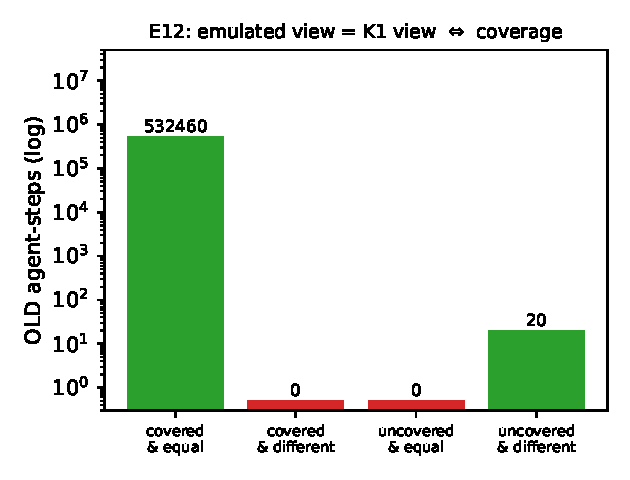
\includegraphics[width=0.45\linewidth]{figs_e3_legacy/fig_e12_coverage.pdf}
\caption{E12: emulated view equals the K1 view iff coverage (532\,480 OLD agent-steps). Green cells agree with Theorem~\ref{thm:emu}; red cells would be exceptions (none observed).}\label{fig:e12}\end{figure}

\subsection{Mixed fleet (E7)}
\begin{table}[t]\centering\small
\begin{tabular}{lrrrr}\toprule
Arm (layout D) & system & OLD & NEW & delivered B/ep\\\midrule
U2 / plain (OLD unaware of the upgrade) & $+1.76\,[0.41, 3.31]$ & $-0.78$ & $+4.30$ & 78\,058\\
U1 / fallback (OLD $\to$ silent student) & $+2.62\,[1.94, 3.22]$ & $+1.85$ & $+3.39$ & 78\,058\\
K1 / rollback & $+1.11\,[-0.34, 2.50]$ & $+1.58$ & $+0.65$ & 10\,400\\
U2 / emulator (0 B) & $+5.76\,[4.49, 6.90]$ & $+5.57$ & $+5.95$ & 78\,058\\
U2 / decoder (+1\,300 B unique) & $+5.76\,[4.49, 6.91]$ & $+5.57$ & $+5.95$ & 78\,058\\
U1 / OLD fine-tuned (FT-mix) & $+5.44\,[4.33, 6.50]$ & $+4.60$ & $+6.28$ & 78\,058\\
U1 / OLD retrained (PCT) & $+5.20\,[4.04, 6.28]$ & $+4.53$ & $+5.87$ & 78\,058\\
all OLD on K1 & $+6.04\,[4.57, 7.21]$ & & & 10\,400\\
all NEW on U1 & $+6.35\,[5.38, 7.22]$ & & & 78\,058\\\bottomrule
\end{tabular}
\caption{E7, layout D: gain (\%) over ZTEAM. Registered endpoints: emulator $-$ fallback $+3.15\,[2.24, 4.07]$ (10/10); emulator $-$
plain $+4.00\,[2.67, 5.33]$ (10/10); NEW-group non-inferiority vs U1/plain with margin 0.5: $+1.91\,[0.91, 3.00]$. Layout C:
$+3.28\,[2.06, 4.58]$, $+3.80\,[2.48, 5.04]$, $+1.32\,[0.34, 2.34]$.}\label{tab:e7}
\end{table}
Table~\ref{tab:e7} gives the primary layout. All three registered endpoints are supported in both layouts. Secondary, two-sided
contrasts:
\begin{itemize}
\item Against update-permitted references the emulator shows no detected difference: $+0.32\,[-0.62, 1.08]$ vs FT-mix and
$+0.56\,[-0.38, 1.25]$ vs PCT (layout D). This is not an equivalence test. A registered confirmation that an outcome-paired variant of
fine-tuning beats FT-mix was not supported ($+0.36\,[-0.17, 0.93]$; E14), so FT-mix and PCT remain the references.
\item The mixed fleet with emulation is slightly \emph{below} retraining the whole fleet: emulator $-$ all-NEW $=-0.59\,[-1.35,-0.02]$
(layout D; layout C $-0.49\,[-1.21, 0.11]$). Against all-OLD on K1 no difference is detected ($-0.27\,[-1.28, 0.48]$).
\item Against rollback, the emulator gains $+4.66\,[3.55, 5.76]$ at 7.5 times the delivered bytes.
\end{itemize}
Figure~\ref{fig:e7} shows every arm with its byte cost.
\begin{figure}[t]\centering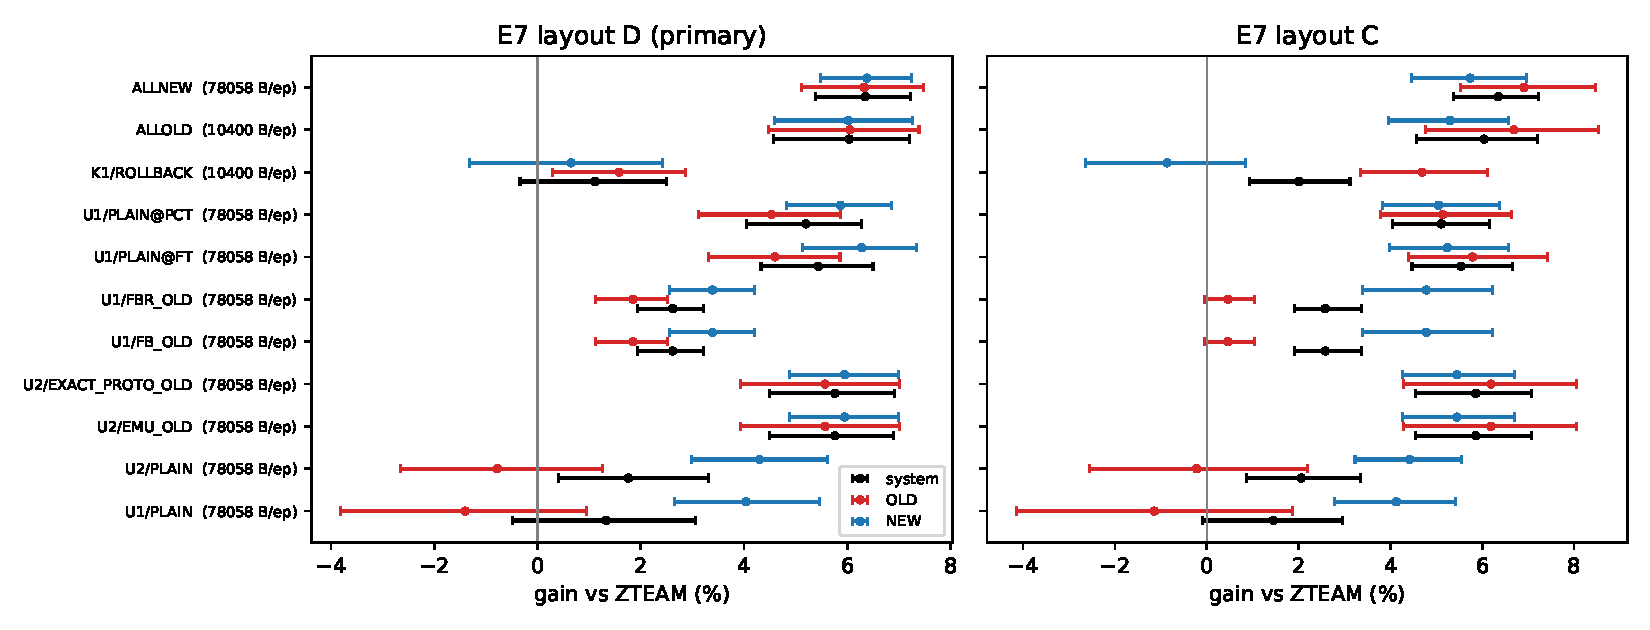
\includegraphics[width=\linewidth]{figs_e3_legacy/fig_e7_arms.pdf}
\caption{E7: system / OLD / NEW gain vs a zero-communication team, per arm, with delivered bytes per episode.}\label{fig:e7}\end{figure}

\subsection{What emulation does not guarantee (E13)}\label{sec:e13}
No OLD agent was significantly worse than in the all-OLD team by more than 0.5 point; all eight point estimates are negative and per-agent
non-inferiority was not established (Bonferroni lower bounds down to $-9.4\%$ in layout D and $-12.9\%$ in layout C). The wide intervals
do not exclude harm of that size; they are not evidence that such harm occurs. Figure~\ref{fig:e13}.
\begin{figure}[t]\centering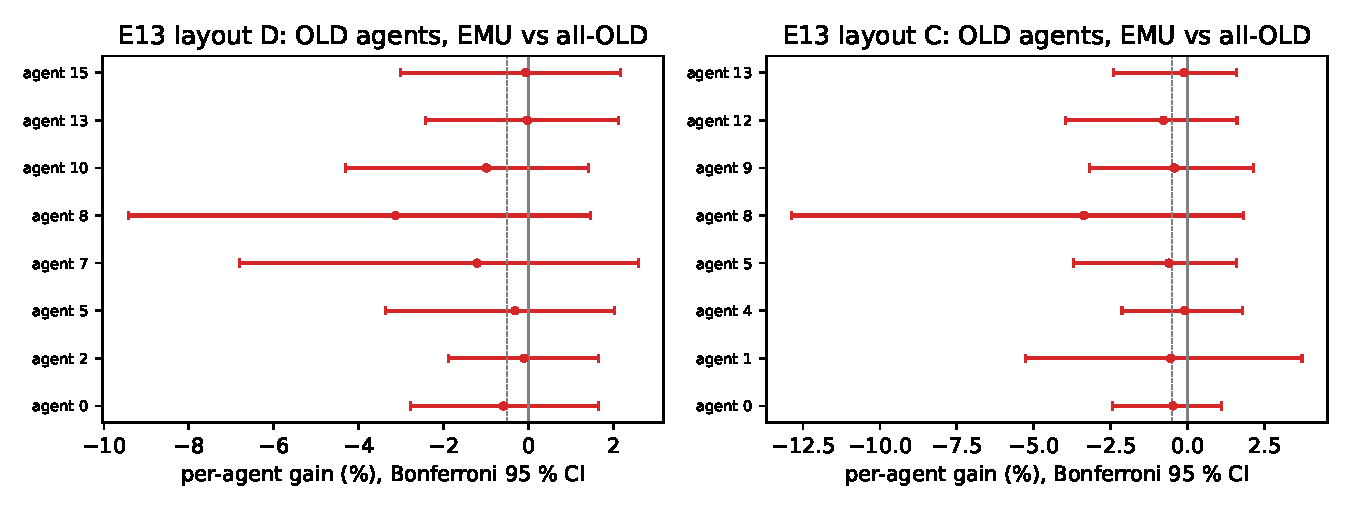
\includegraphics[width=0.9\linewidth]{figs_e3_legacy/fig_e13_forest.pdf}
\caption{E13: per-OLD-agent gain vs all-OLD with Bonferroni 95\% intervals.}\label{fig:e13}\end{figure}

\section{Related work}
\paragraph{Specification and refinement.} Our decoder lemma is a refinement/simulation argument in the sense of Abadi and Lamport;
behavioural subtyping with history properties (Liskov and Wing) and agent-to-agent protocols with task lifecycles already treat history,
not only formats. The tool is standard; the object --- the view on which a frozen \emph{learned} receiver was trained --- is ours.
\paragraph{Backward-compatible model updates.} An updated component can hurt a frozen consumer (Bansal et al.\ 2019); backward-compatible
training (Shen et al.\ 2020) and positive-congruent training (Yan et al.\ 2021) change the \emph{new} model. Our emulators leave every
model unchanged and repair the channel; PCT appears as a reference arm.
\paragraph{Delay- and channel-robust MARL communication.} Delay compensation (RDC, NeurIPS 2025), information-gap bounds (CGDC), and
learned waiting (DACOM) train or adapt receivers; we keep receivers frozen.
\paragraph{Consistent network updates.} Per-packet consistency (Reitblatt et al.\ 2012) guarantees that each packet sees one configuration;
our contract guarantees that each frozen receiver sees one \emph{view}.

\section{Limitations}
Same-trajectory guarantee only; honesty of copies is assumed; one simulator and one grid; an external benchmark is pending (download
permission). The emulator's guarantee is conditional on coverage, which is a property of the channel realisation; the decoder costs
bytes. The fleet with emulation remains slightly below a fully retrained fleet.

\section*{Provenance}
Every number: claim table rows C1--C6 (report line, producer hash, manifest status COMPLETE / self\_check PASS).

\appendix
\section{Reproducibility}
\begin{tabular}{lll}\toprule
Result & Producer (sha256 prefix) & Report\\\midrule
E9 decoder replay & \texttt{MARL\_e3\_legacy\_decoder\_nodes\_eval.py} 2d268743 & \texttt{e9\_report.txt} (\texttt{MARL\_e3\_e9\_report.py} 13aadb17)\\
E12 coverage & \texttt{MARL\_e3\_emu\_coverage\_eval.py} b4964c67 & \texttt{e12/report.txt} (\texttt{MARL\_e3\_e12\_report.py} f73b7825)\\
E7 mixed fleet & \texttt{MARL\_e3\_mixed\_fleet\_eval\_v2.py} b656a1f6 & \texttt{w2/report\_e7.txt} (\texttt{MARL\_e3\_wave2\_report.py} bb36f5af)\\
E14 & --- & \texttt{MARL\_e3\_e14\_report.py} bcd16643\\
Lean decoder & \lean{LeanMarlLegacyViewDecoderV1} & smoke gate, 21 theorems, standard axioms\\
Lean emulator & \lean{LeanMarlPacketEmulatorV1} & smoke gate, 10 theorems, standard axioms\\\bottomrule
\end{tabular}

\noindent Self-checks run on the first episode of every evaluation and block the manifest if they fail: a homogeneous OLD team with the
decoder equals the K1 run; a team with no OLD agent equals the homogeneous NEW run; the zero-communication arm equals the separately
computed ZTEAM run; per-agent queues sum to the step queue.

\end{document}
